\begin{figure}[!]
    \centering
    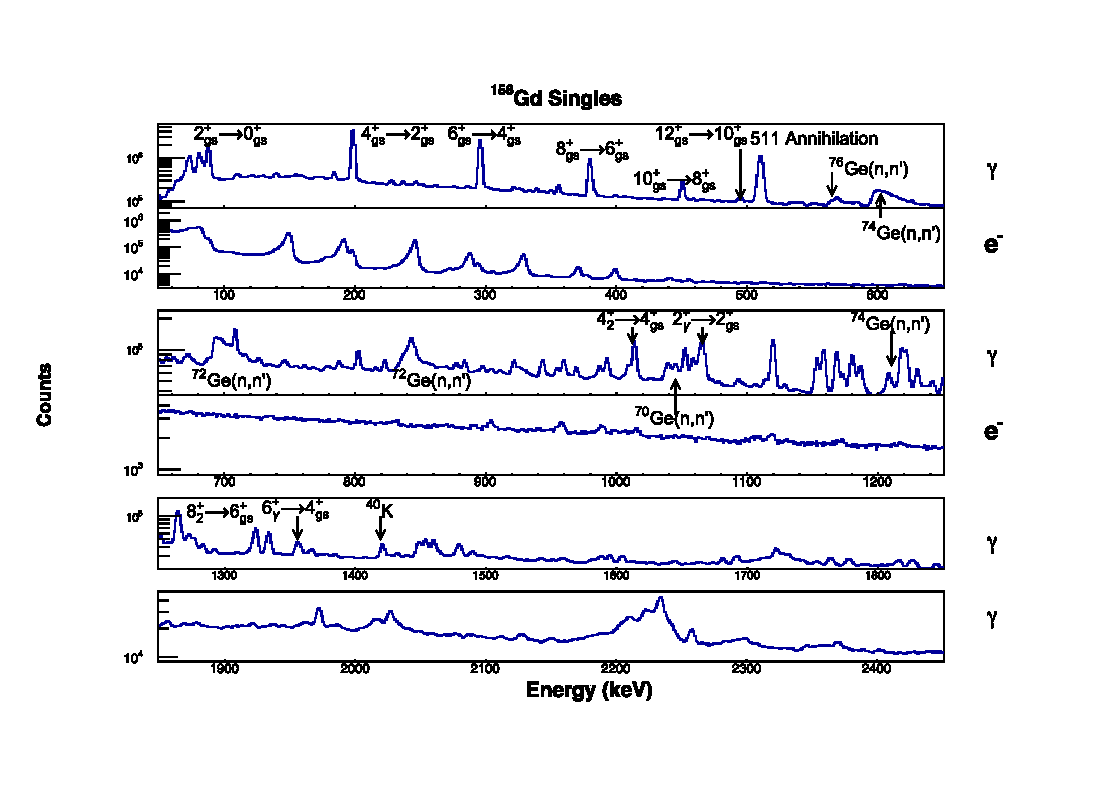
\includegraphics[scale=0.9]{156GdTablesAndFigs/156Gd_Singles_Label.eps}
    \caption{Singles spectra of $^{156}$Gd. Spectra are labeled with the particles being detected, the energies of the $\gamma$ and electron spectra aligned for identification. In the $\gamma$ spectrum, several lines of note are labeled. These are the ground-state band lines as well as other transitions of interest. Below 100 keV is a combination of x-rays and the 89 keV gamma from the ground state band. In the conversion electron spectrum, the large peaks up to approximately 350 keV are from the ground state band. These large peaks make the ground state band a good diagnostic, but also emphasize the need for coincidence gating, as the conversion electron spectrum is flooded by the ground state band electrons. The large peak at low energy is cut off due to the threshold. It is a combination of background and the 89L peak. Transitions in the higher energy regime of the $\gamma$ spectrum cannot be determined without gating, due to additional background from the experimental room.}
    \label{fig:156_Singles}
\end{figure}